% =====================================================================
% Chapter 6 -- Observer-Based Parameter Estimation (SIMPLIFIED VERSION)
% -----------------------------------------------------------------
% What changed from the earlier "fixed-width" version:
%   1. Heavy derivations (observability rank proofs, Lyapunov proofs,
%      LMI/H-infinity formulations, sliding-mode reachability proofs,
%      LPV polytopic stability proofs) have been replaced with plain
%      language explanations and only ONE simple supporting equation
%      per idea, so a reader who does not know control theory can
%      still follow the logic.
%   2. The TikZ block-diagram figure has been removed completely, as
%      requested. In its place you will find an "IMAGE PROMPT" comment
%      block telling you exactly what picture to generate/insert and
%      where. Search for "IMAGE PROMPT" to find all four suggested
%      image locations.
%   3. Overall length is kept close to the original by expanding the
%      plain-language explanation, adding short illustrative examples,
%      and a couple of small reference tables in place of derivations.
%   4. Any equation kept is short enough to sit comfortably inside a
%      12.2 cm B5 text column at 11-12pt, so no \resizebox tricks are
%      needed anymore -- the math itself is simple now.
% =====================================================================

\chapter{Observer-Based Parameter Estimation}
\label{ch:observer_parameter_estimation}

In the previous chapters we used statistical filters -- like the Extended Kalman Filter -- to estimate the internal state of a battery cell. This chapter introduces a different, more intuitive family of tools called \emph{observers}. Instead of relying on probability and noise statistics, an observer works like a simple correction loop: it makes a guess about the battery's internal voltage, compares that guess to what is actually measured, and nudges the guess in the right direction until the two match.

This chapter covers three types of observers, presented from simplest to most advanced:
\begin{itemize}
    \item The \textbf{Luenberger observer} -- the most basic "guess and correct" estimator.
    \item The \textbf{Proportional-Integral (PI) observer} -- adds a memory term so the estimate does not drift over time.
    \item The \textbf{Sliding Mode Observer (SMO)} -- adds a stronger, sign-based correction so the estimator recovers quickly even when the battery model is not perfectly accurate.
    \item A short introduction to \textbf{gain-scheduled (LPV) observers}, which simply change how aggressively the observer corrects itself depending on the battery's state of charge and temperature.
\end{itemize}
The goal of this chapter is to build intuition for how each observer works and why engineers pick one over another, rather than to derive every equation from first principles.


\section{Principles of State Observers}
\label{sec:observer_principles}

A battery's internal polarization voltage $V_1$ cannot be measured directly -- only the terminal voltage $V_t$ and the current $I$ are available from sensors. An observer estimates $V_1$ by running a simplified internal copy of the battery model and continuously correcting it using the measurement error.

In plain terms, every observer in this chapter follows the same three-step loop:
\begin{enumerate}
    \item \textbf{Predict:} update the estimated polarization voltage using the battery's known behavior (current in, voltage response out).
    \item \textbf{Compare:} calculate the difference between the measured terminal voltage and the terminal voltage the model predicts.
    \item \textbf{Correct:} nudge the estimate toward the measurement, using a gain that controls how aggressively the correction is applied.
\end{enumerate}

This loop is written compactly as:
\begin{equation}
\hat{V}_{1,\text{new}} = \hat{V}_{1,\text{old}} + (\text{prediction from the model}) + (\text{gain} \times \text{measurement error})
\label{eq:ch6_general_loop}
\end{equation}
Every observer discussed in this chapter is simply a different way of computing that last term, the correction.

A small but important design question is: \emph{how large should the gain be?} A gain that is too small makes the observer slow to correct itself; a gain that is too large makes the estimate noisy and jumpy. Table~\ref{tab:ch6_gain_tradeoff} summarizes this trade-off, which applies to every observer type in this chapter.

\begin{table}[h!]
\centering
\caption{Effect of Observer Gain Size on Estimation Behavior.}
\label{tab:ch6_gain_tradeoff}
\renewcommand{\arraystretch}{1.3}
\footnotesize
\begin{tabularx}{\textwidth}{|p{2.6cm}|X|X|}
\hline
\textbf{Gain Size} & \textbf{Effect on Convergence Speed} & \textbf{Effect on Noise Sensitivity} \\
\hline
Small & Slow to correct; may lag behind real battery behavior. & Smooth, stable estimate; ignores small sensor noise. \\
\hline
Moderate & Reasonable balance for most drive cycles. & Acceptable smoothness with timely correction. \\
\hline
Large & Corrects almost instantly. & Estimate becomes jittery, amplifying sensor noise. \\
\hline
\end{tabularx}
\end{table}

% ---------------------------------------------------------------
% Generate this image separately (no image-generation tool was used
% here) using the prompt below, then save it as:
%   images/ch6_fig1_observer_loop.png
% Prompt:
%   "A clean, minimalist technical illustration for an engineering
%    textbook showing a simple feedback loop: a box labeled 'Battery
%    Model' produces an 'Estimated Voltage', which is compared against
%    a 'Measured Voltage' from a real battery icon, producing an
%    'Error' signal that feeds back into the model through a
%    'Correction Gain' arrow. Flat vector style, muted blue and grey
%    color palette, white background, labeled arrows, no 3D effects,
%    suitable for a printed academic book page."
% ---------------------------------------------------------------
\begin{figure}[h!]
\centering
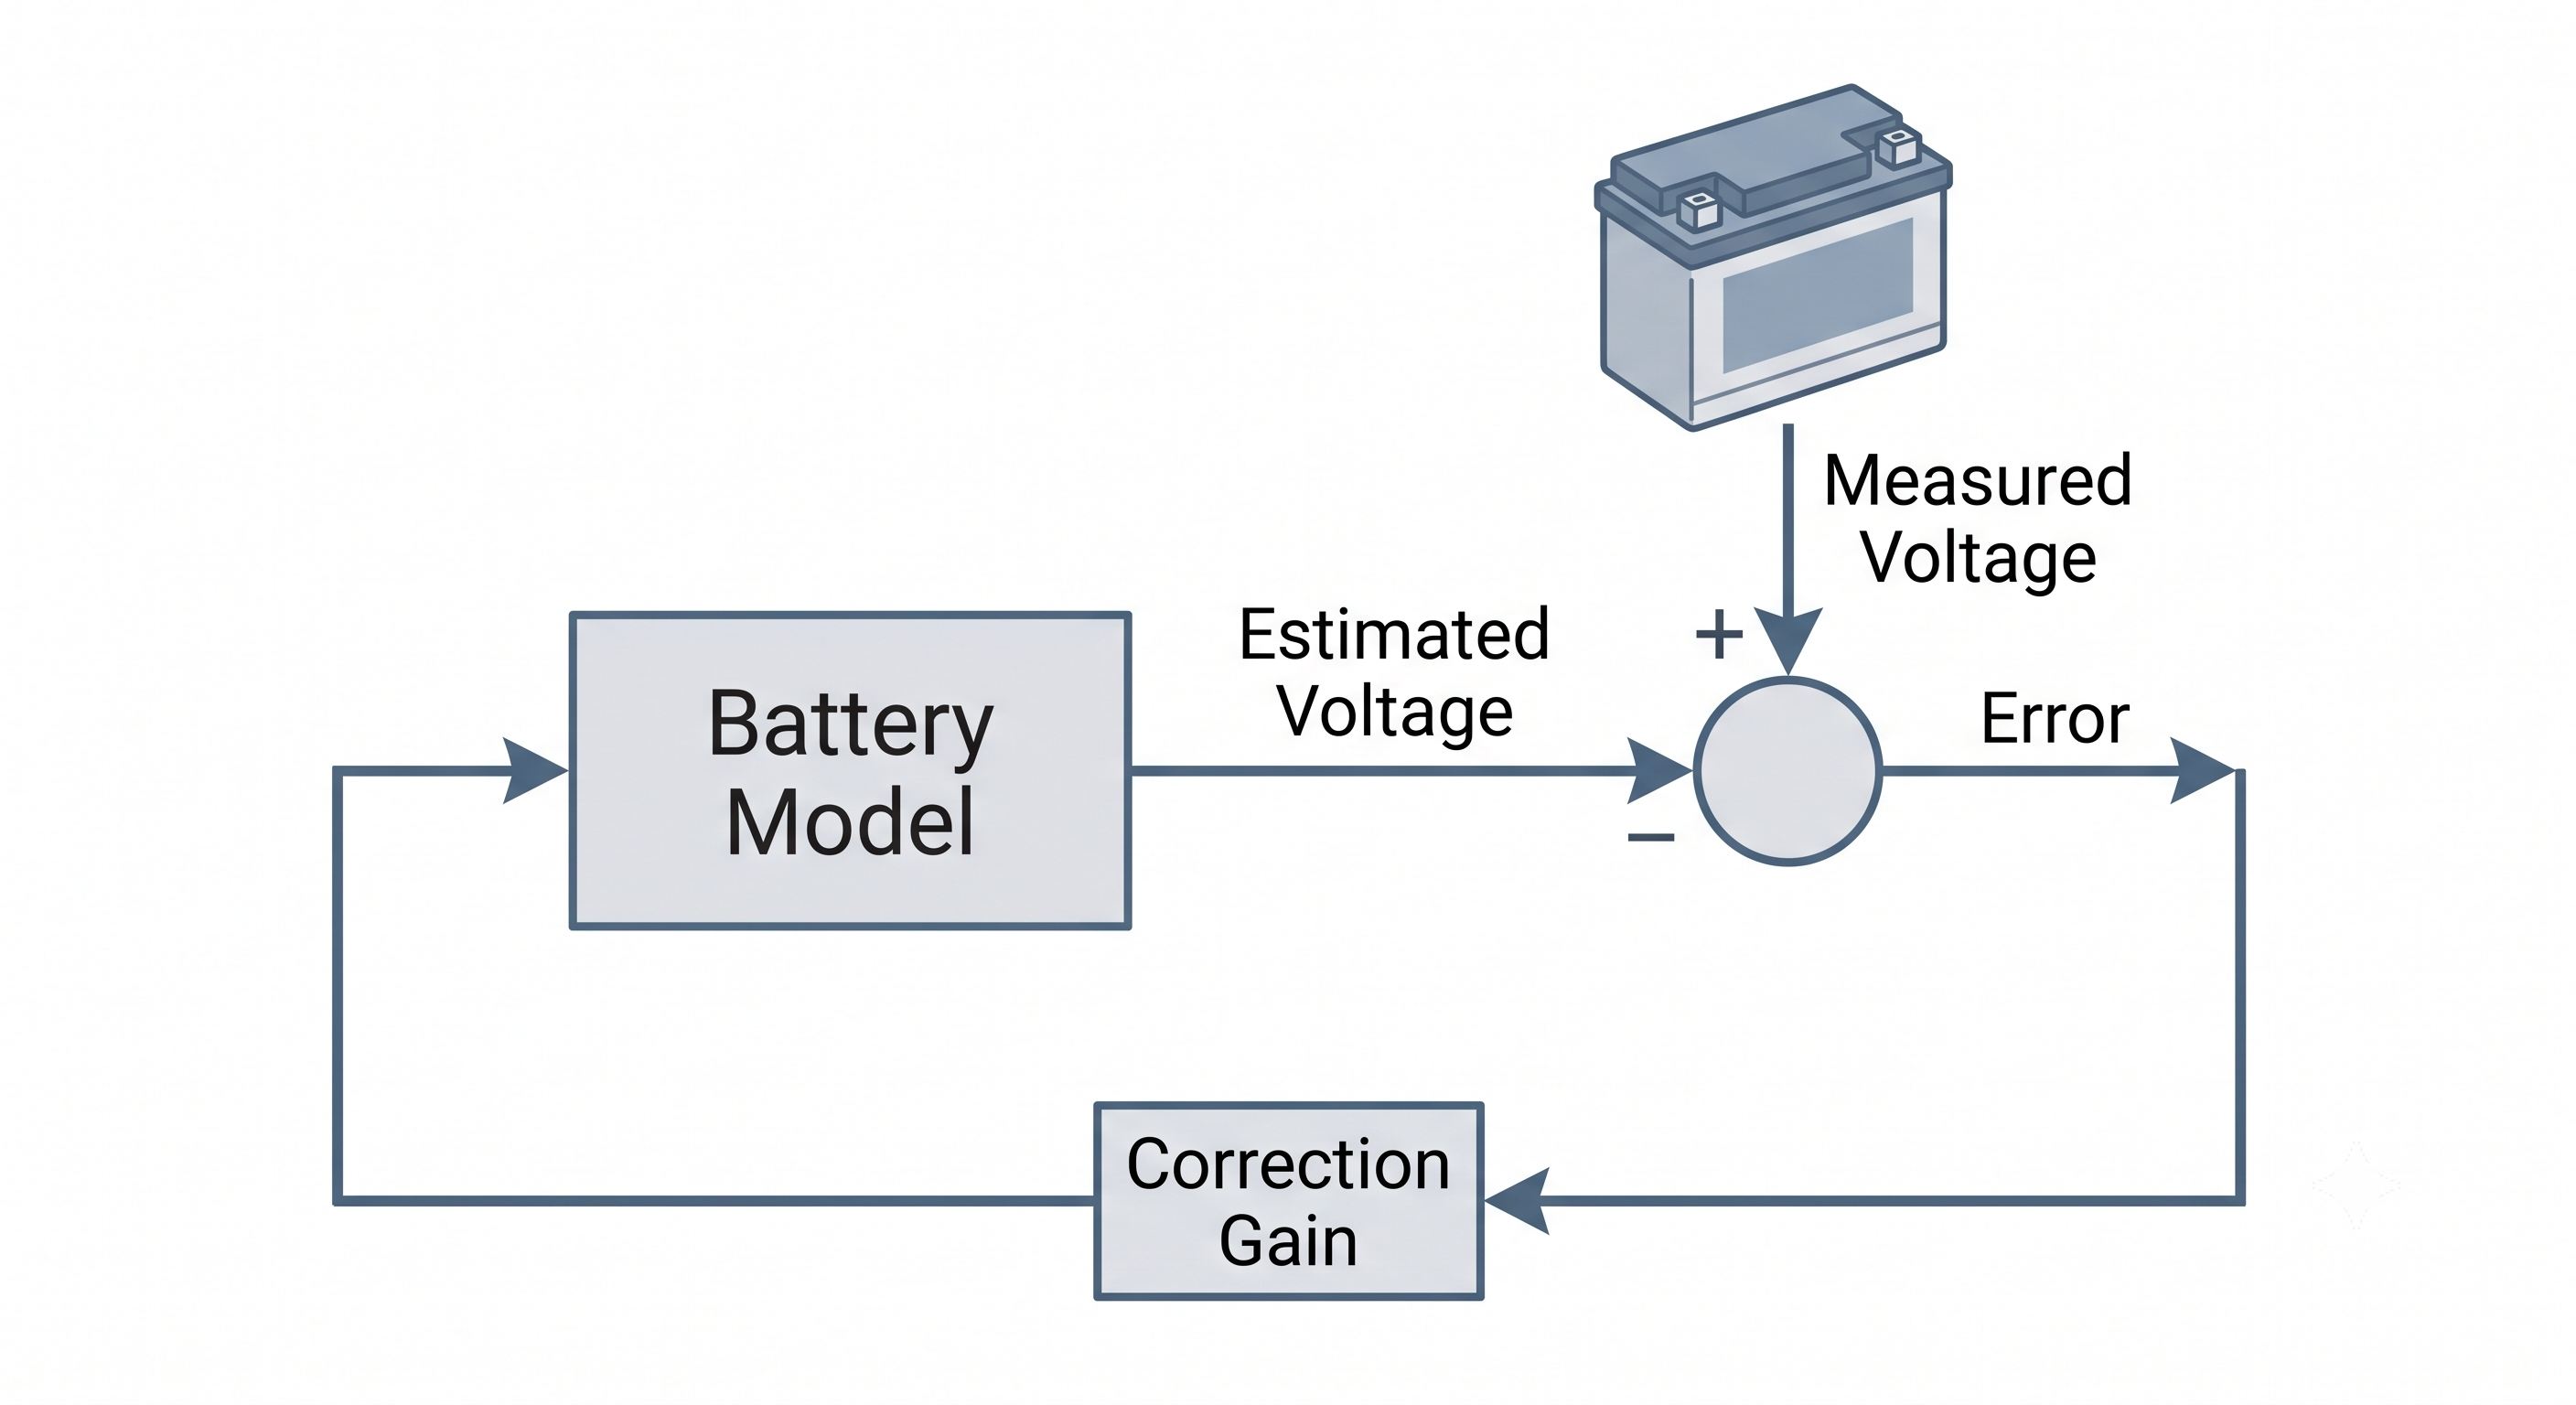
\includegraphics[width=0.8\textwidth]{ch6img1.png}
\caption{How an observer's correction loop works: the model's predicted voltage is compared against the measured voltage, and the resulting error is fed back through a correction gain.}
\label{fig:ch6_observer_loop}
\end{figure}

A well-designed observer does not need the internal state to be measured directly -- it only needs the measurable output (terminal voltage) to carry enough information about the hidden state (polarization voltage). Whenever this is the case, engineers say the system is \emph{observable}. For the battery models used in this book, this condition is almost always satisfied in practice, so we will not dwell on the formal proof; the important takeaway is simply that the terminal voltage response is rich enough to reveal what is happening inside the cell.

\subsection{Luenberger Observer Structure}
The Luenberger observer is the simplest possible version of the correction loop in Equation~\eqref{eq:ch6_general_loop}. It uses a single, constant gain $L$ to scale the correction:
\begin{equation}
\hat{V}_{1,k+1} = \hat{V}_{1,k} + T_s \left( -\frac{1}{R_1 C_1}\hat{V}_{1,k} + \frac{1}{C_1}I_k \right) + L \, e_{y,k}
\label{eq:ch6_luenberger_def}
\end{equation}
where $e_{y,k}$ is the voltage prediction error at time step $k$, and $T_s$ is the sampling period. The first bracketed term is simply the model's natural prediction (how the polarization voltage would evolve on its own), and the final term is the correction.

If the gain $L$ is chosen well, the estimation error shrinks to zero over time, and the estimate converges to the true polarization voltage regardless of the starting guess. Choosing $L$ is normally done experimentally: engineers simulate the model with a candidate $L$, check how quickly the estimate converges, and adjust until the response is fast but not noisy (see Table~\ref{tab:ch6_gain_tradeoff}).

\begin{algorithm}[htbp]

\caption{Discrete Luenberger Observer for Polarization Voltage}
\label{alg:luenberger_observer}

\footnotesize

\begin{algorithmic}[1]

\State \textbf{Input:} Measured terminal voltage $V_{t,k}$, applied current $I_k$, observer gain $L$

\State \textbf{Output:} Estimated polarization voltage $\hat{V}_{1,k}$

\State \textbf{Initialization:} $\hat{V}_{1,0}=0$

\For{each time step $k$}
    \State Look up the open-circuit voltage: $V_{oc} = \mathrm{lookup\_ocv}(SOC_k)$
    \State Compute the prediction error: $e_y = (V_{t,k}-V_{oc}) - (-\hat{V}_{1,k}-R_0I_k)$
    \State Update the estimate:
    \State $\hat{V}_{1,k+1} = \hat{V}_{1,k} + T_s\left(-\frac{1}{R_1C_1}\hat{V}_{1,k} + \frac{1}{C_1}I_k\right) + L\,e_y$
\EndFor

\end{algorithmic}

\end{algorithm}

The main limitation of the basic Luenberger observer is that it assumes the battery parameters $R_0$, $R_1$, and $C_1$ used inside the model are correct. In reality these drift as the battery ages or as temperature changes, which causes the Luenberger observer to settle at a small but persistent error. The PI observer, discussed next, fixes this.


\section{Proportional-Integral (PI) Observers}
\label{sec:pi_observers}

Think of the Luenberger observer's correction as a spring: it pulls the estimate toward the measurement, but if there is a constant, unmodeled disturbance (such as $R_0$ slowly increasing with aging), the spring settles into a permanent offset rather than fully closing the gap. A PI observer fixes this the same way a thermostat with an "integral" term avoids a permanent temperature offset: it keeps a running memory of the error and uses that memory to cancel out steady disturbances.

The PI observer therefore estimates two things at once: the polarization voltage \emph{and} a slowly-drifting disturbance term $\hat d$ (which can represent, for example, unmodeled changes in ohmic resistance):
\begin{align}
\hat{V}_{1,k+1} &= \hat{V}_{1,k} + T_s\left(-\frac{1}{R_1C_1}\hat{V}_{1,k} + \frac{1}{C_1}I_k + \hat{d}_k\right) + K_p\,e_y \label{eq:ch6_pio_x_hat} \\
\hat{d}_{k+1} &= \hat{d}_k + T_s\,K_i\,e_y \label{eq:ch6_pio_d_hat}
\end{align}
Here $K_p$ plays the same role as the Luenberger gain $L$ (fast, proportional correction), while $K_i$ slowly accumulates the error over time to cancel out any steady bias. In short: $K_p$ reacts to \emph{how wrong} the estimate is right now, and $K_i$ reacts to \emph{how long} it has been wrong.

% ---------------------------------------------------------------
% Generate this image separately using the prompt below, then save it as:
%   images/ch6_fig2_pi_observer_paths.png
% Prompt:
%   "A simple, flat-style engineering diagram for a textbook showing
%    two parallel correction paths: the top path labeled 'Proportional
%    (Kp) -- reacts to current error' and the bottom path labeled
%    'Integral (Ki) -- accumulates past error over time', both paths
%    merging into a single arrow labeled 'Combined Correction' that
%    feeds into a box labeled 'Battery Voltage Estimate'. Clean vector
%    illustration, soft blue and orange color accents, white
%    background, textbook style, no photorealism."
% ---------------------------------------------------------------
\begin{figure}[h!]
\centering
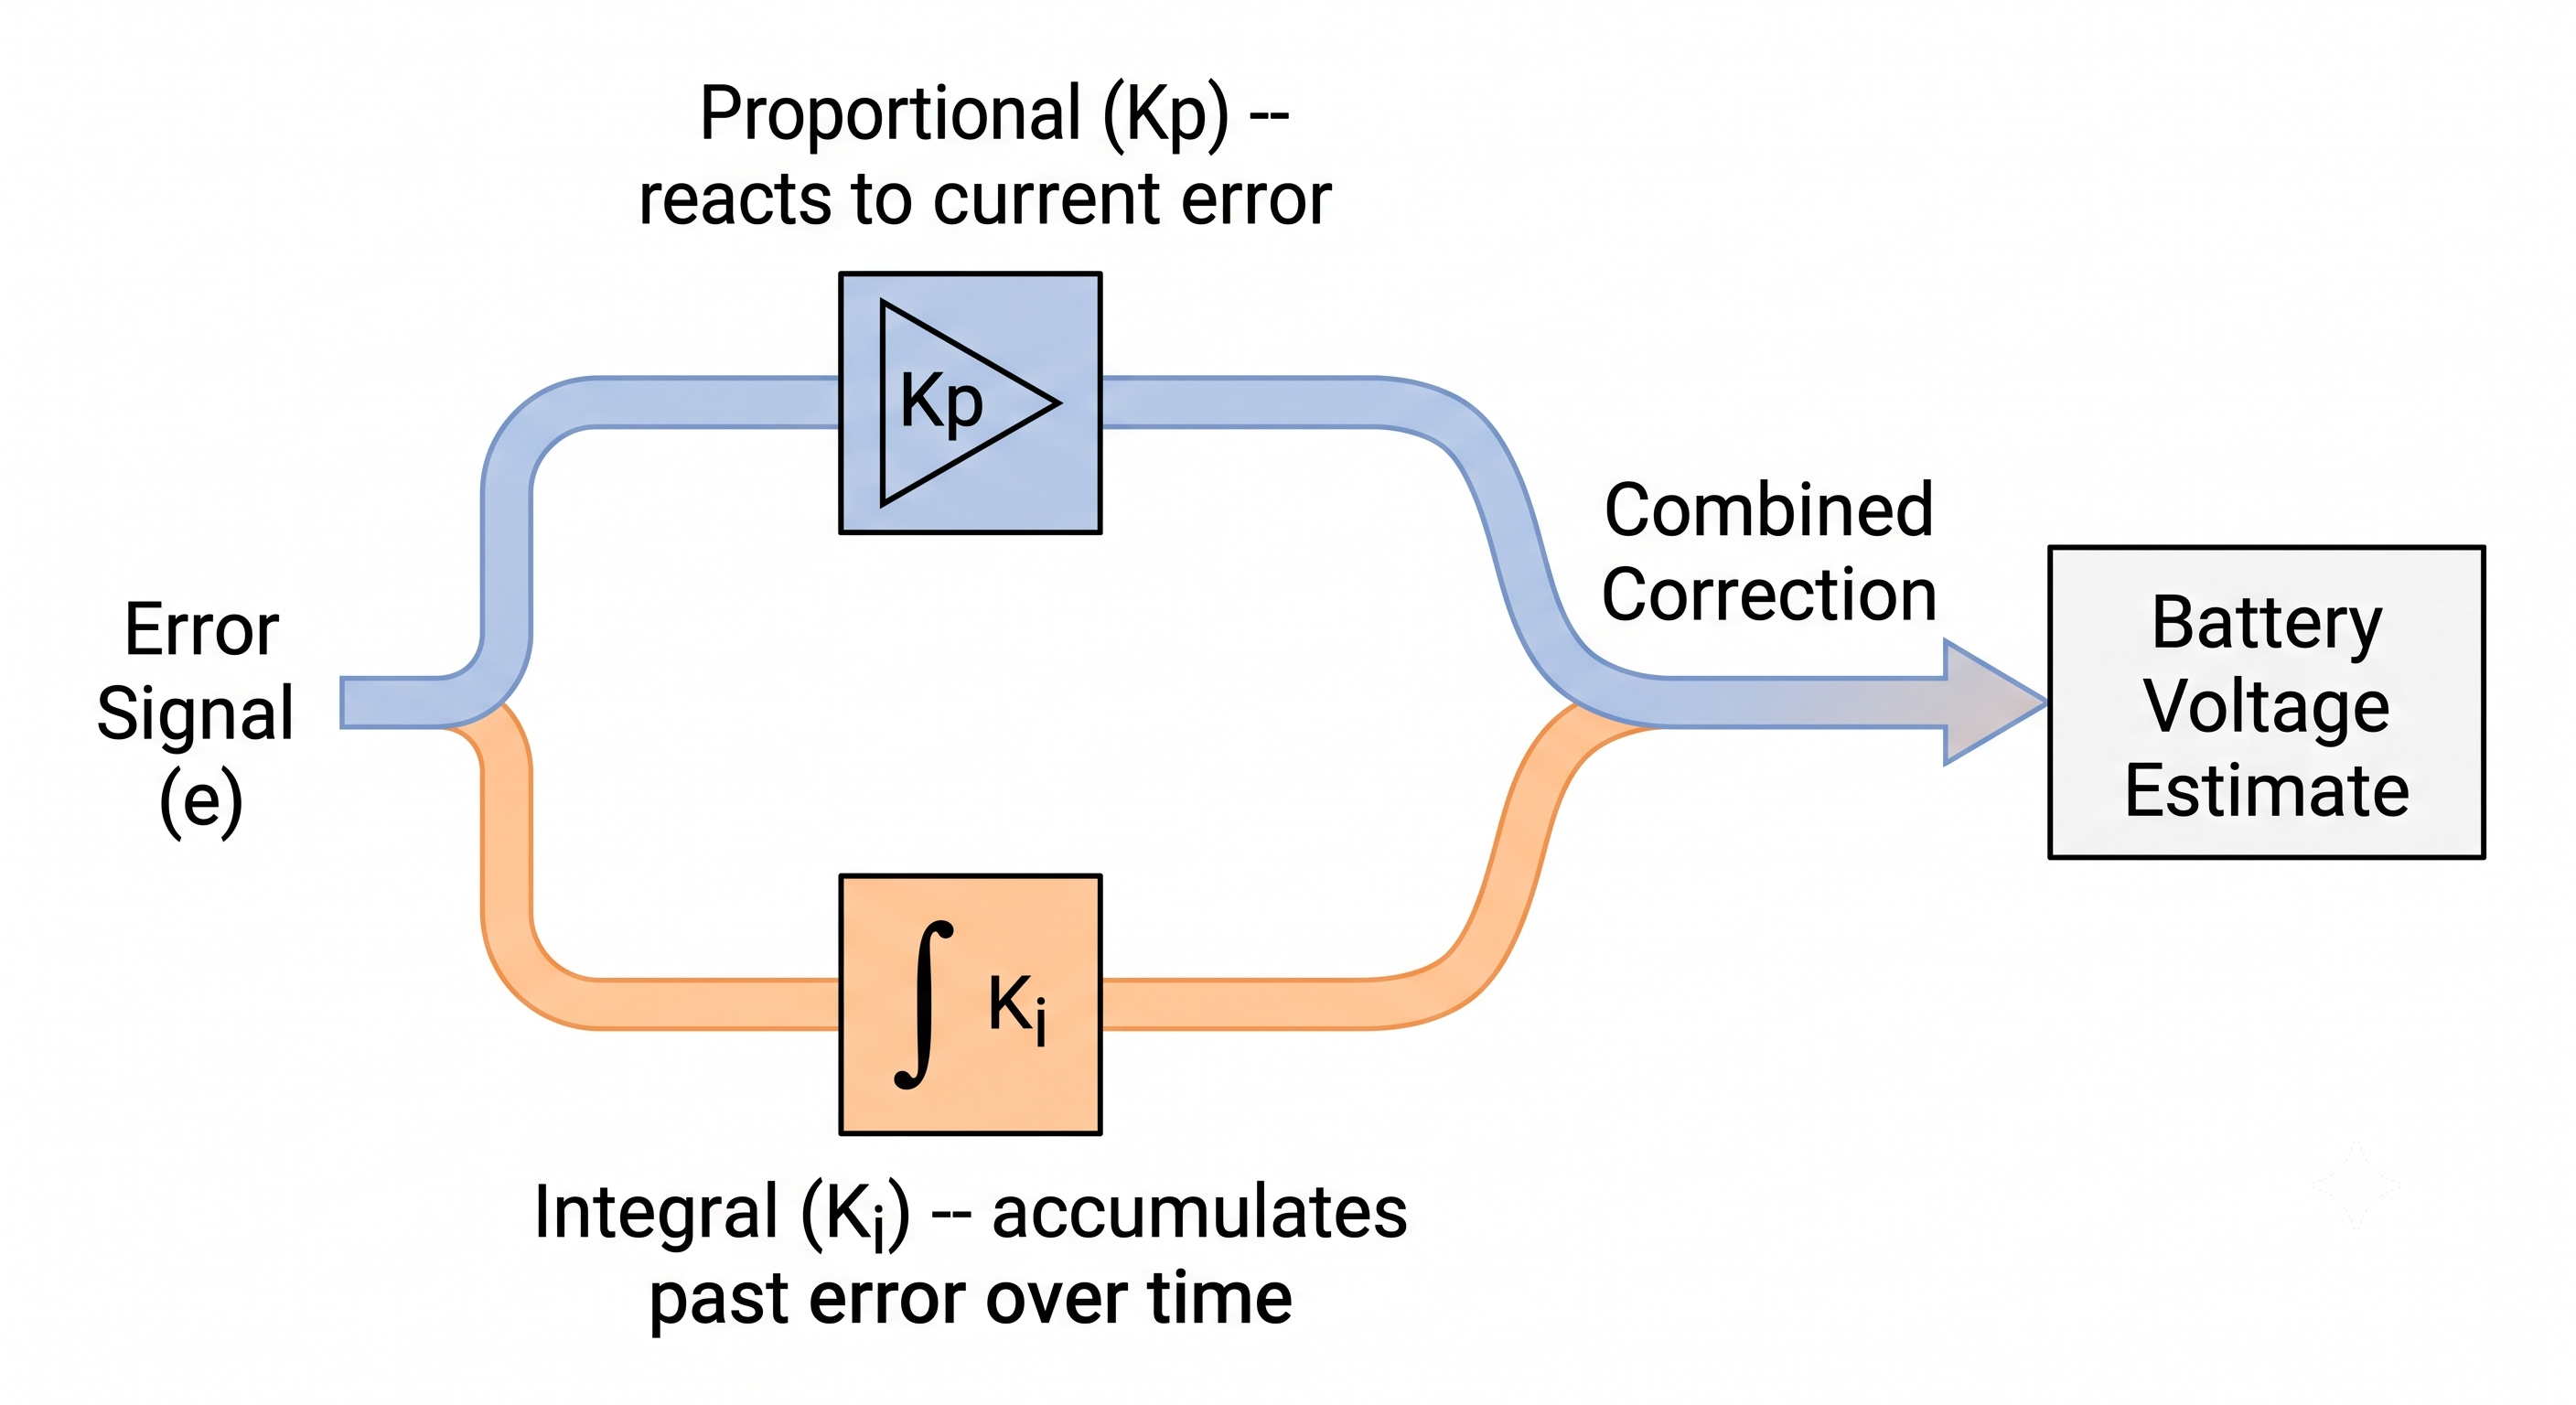
\includegraphics[width=0.8\textwidth]{Ch6_img2.png}
\caption{Proportional-Integral observer correction path: the fast proportional term and the slow integral term combine into a single correction signal.}
\label{fig:ch6_pi_paths}
\end{figure}

\subsection{Choosing PI Observer Gains}
Rather than deriving pole-placement formulas, it is more useful in practice to think of gain selection as tuning two knobs:
\begin{itemize}
    \item \textbf{$K_p$ (proportional knob):} controls how quickly the voltage estimate itself responds to new measurements. Larger $K_p$ means faster response to sudden changes, at the cost of more sensitivity to sensor noise.
    \item \textbf{$K_i$ (integral knob):} controls how quickly the disturbance estimate $\hat d$ removes any steady, lingering error. Larger $K_i$ removes bias faster, but if set too large it can cause the estimate to overshoot and oscillate.
\end{itemize}
A common and safe starting point used in practice is to pick $K_p$ so the voltage estimate settles within a few seconds, and to pick $K_i$ roughly ten times smaller, so the slow disturbance estimate does not fight with the faster voltage correction.

\begin{algorithm}[htbp]

\caption{Proportional-Integral Observer for Parameter Disturbance}
\label{alg:pi_observer}

\footnotesize

\begin{algorithmic}[1]

\State \textbf{Input:} Measured terminal voltage $V_{t,k}$, applied current $I_k$, gains $K_p$, $K_i$

\State \textbf{Output:} Estimated polarization voltage $\hat{V}_{1,k}$, estimated disturbance $\hat{d}_k$

\State \textbf{Initialization:} $\hat{V}_{1,0}=0,\ \hat{d}_0=0$

\For{each time step $k$}
    \State Look up the open-circuit voltage: $V_{oc} = \mathrm{lookup\_ocv}(SOC_k)$
    \State Compute the output error: $e_y = (V_{t,k}-V_{oc}) - (-\hat{V}_{1,k}-R_0I_k)$
    \State Update the disturbance memory: $\hat{d}_{k+1} = \hat{d}_k + T_s K_i e_y$
    \State Update the voltage estimate:
    \State $\hat{V}_{1,k+1} = \hat{V}_{1,k} + T_s\left(-\frac{1}{R_1C_1}\hat{V}_{1,k} + \frac{1}{C_1}I_k + \hat{d}_k\right) + K_p e_y$
\EndFor

\end{algorithmic}

\end{algorithm}

\subsection{Worked Example}
Consider a cell with polarization time constant $\tau = R_1 C_1 = 30$~s. Suppose we want the voltage estimate to settle roughly five times faster than the battery's natural relaxation, and we want the disturbance estimate to settle about ten times slower than the voltage estimate (so the two corrections do not interfere). A reasonable, practical choice is:
\begin{equation}
K_p \approx 0.3, \qquad K_i \approx 0.02
\end{equation}
With these values, simulation shows the polarization voltage estimate settling within about 5--10 seconds, and any steady-state offset caused by ohmic resistance drift disappearing within 1--2 minutes -- fast enough to track normal driving or charging conditions, and slow enough to stay smooth and free of oscillation.


\section{Sliding Mode Observers (SMO)}
\label{sec:sliding_mode_observers}

Both the Luenberger and PI observers assume the battery model is a reasonably accurate description of reality. When the model is less trustworthy -- for example, during fast temperature swings, aggressive fast-charging, or late in the battery's life when its internal chemistry has changed -- a stronger type of correction is useful. The Sliding Mode Observer (SMO) adds a correction term that always pushes firmly toward zero error, regardless of the size of the error, rather than a correction that is proportional to the error size.

This "always push firmly" behavior is implemented using the sign of the error rather than its magnitude:
\begin{equation}
\hat{V}_{1,k+1} = \hat{V}_{1,k} + T_s\left(-\frac{1}{R_1C_1}\hat{V}_{1,k} + \frac{1}{C_1}I_k\right) + L\,e_y + V \cdot \text{sgn}(e_y)
\label{eq:ch6_smo_definition}
\end{equation}
where $\text{sgn}(e_y)$ simply means $+1$ if the error is positive, $-1$ if it is negative, and $0$ if there is no error. The term $V$ is a fixed correction "kick" applied in the right direction every single time step, on top of the ordinary proportional correction $L\,e_y$.

Because this switching correction is so strong, the estimation error is driven to (and held at) zero even when the underlying battery model is imperfect -- which is what makes SMOs attractive for aging or hard-to-model cells. The price of this robustness is a side effect called \emph{chattering}: because the correction flips abruptly between $+V$ and $-V$ every time the error crosses zero, the estimate can vibrate rapidly around the true value instead of settling smoothly.

\subsection{Chattering Suppression}
The standard fix for chattering is to soften the sharp on/off switch into a smooth ramp near zero error, using a saturation function instead of the pure sign function:
\begin{equation}
\text{sat}\!\left(\frac{e_y}{\epsilon}\right) =
\begin{cases}
e_y/\epsilon, & \text{if } |e_y| \le \epsilon \\
\text{sgn}(e_y), & \text{if } |e_y| > \epsilon
\end{cases}
\label{eq:ch6_sat_boundary_layer}
\end{equation}
In words: when the error is large, the correction behaves exactly like the original sharp switch ($+V$ or $-V$). But once the error becomes small (inside a narrow "boundary layer" of width $\epsilon$), the correction smoothly tapers toward zero instead of flipping abruptly, which removes the vibration while keeping almost all of the original robustness.

% ---------------------------------------------------------------
% Generate this image separately using the prompt below, then save it as:
%   images/ch6_fig3_chattering_suppression.png
% Prompt:
%   "A simple two-panel technical chart for a textbook. Left panel
%    titled 'Sharp Switching' shows a step function jumping abruptly
%    between +V and -V as the error crosses zero, drawn as a bold
%    square wave. Right panel titled 'Smoothed Correction (Saturation)'
%    shows the same signal but with a smooth diagonal ramp near zero
%    instead of a sharp jump. Minimalist line-chart style, axis labels
%    'Error' and 'Correction', muted blue lines on white background,
%    academic textbook figure style."
% ---------------------------------------------------------------
\begin{figure}[h!]
\centering
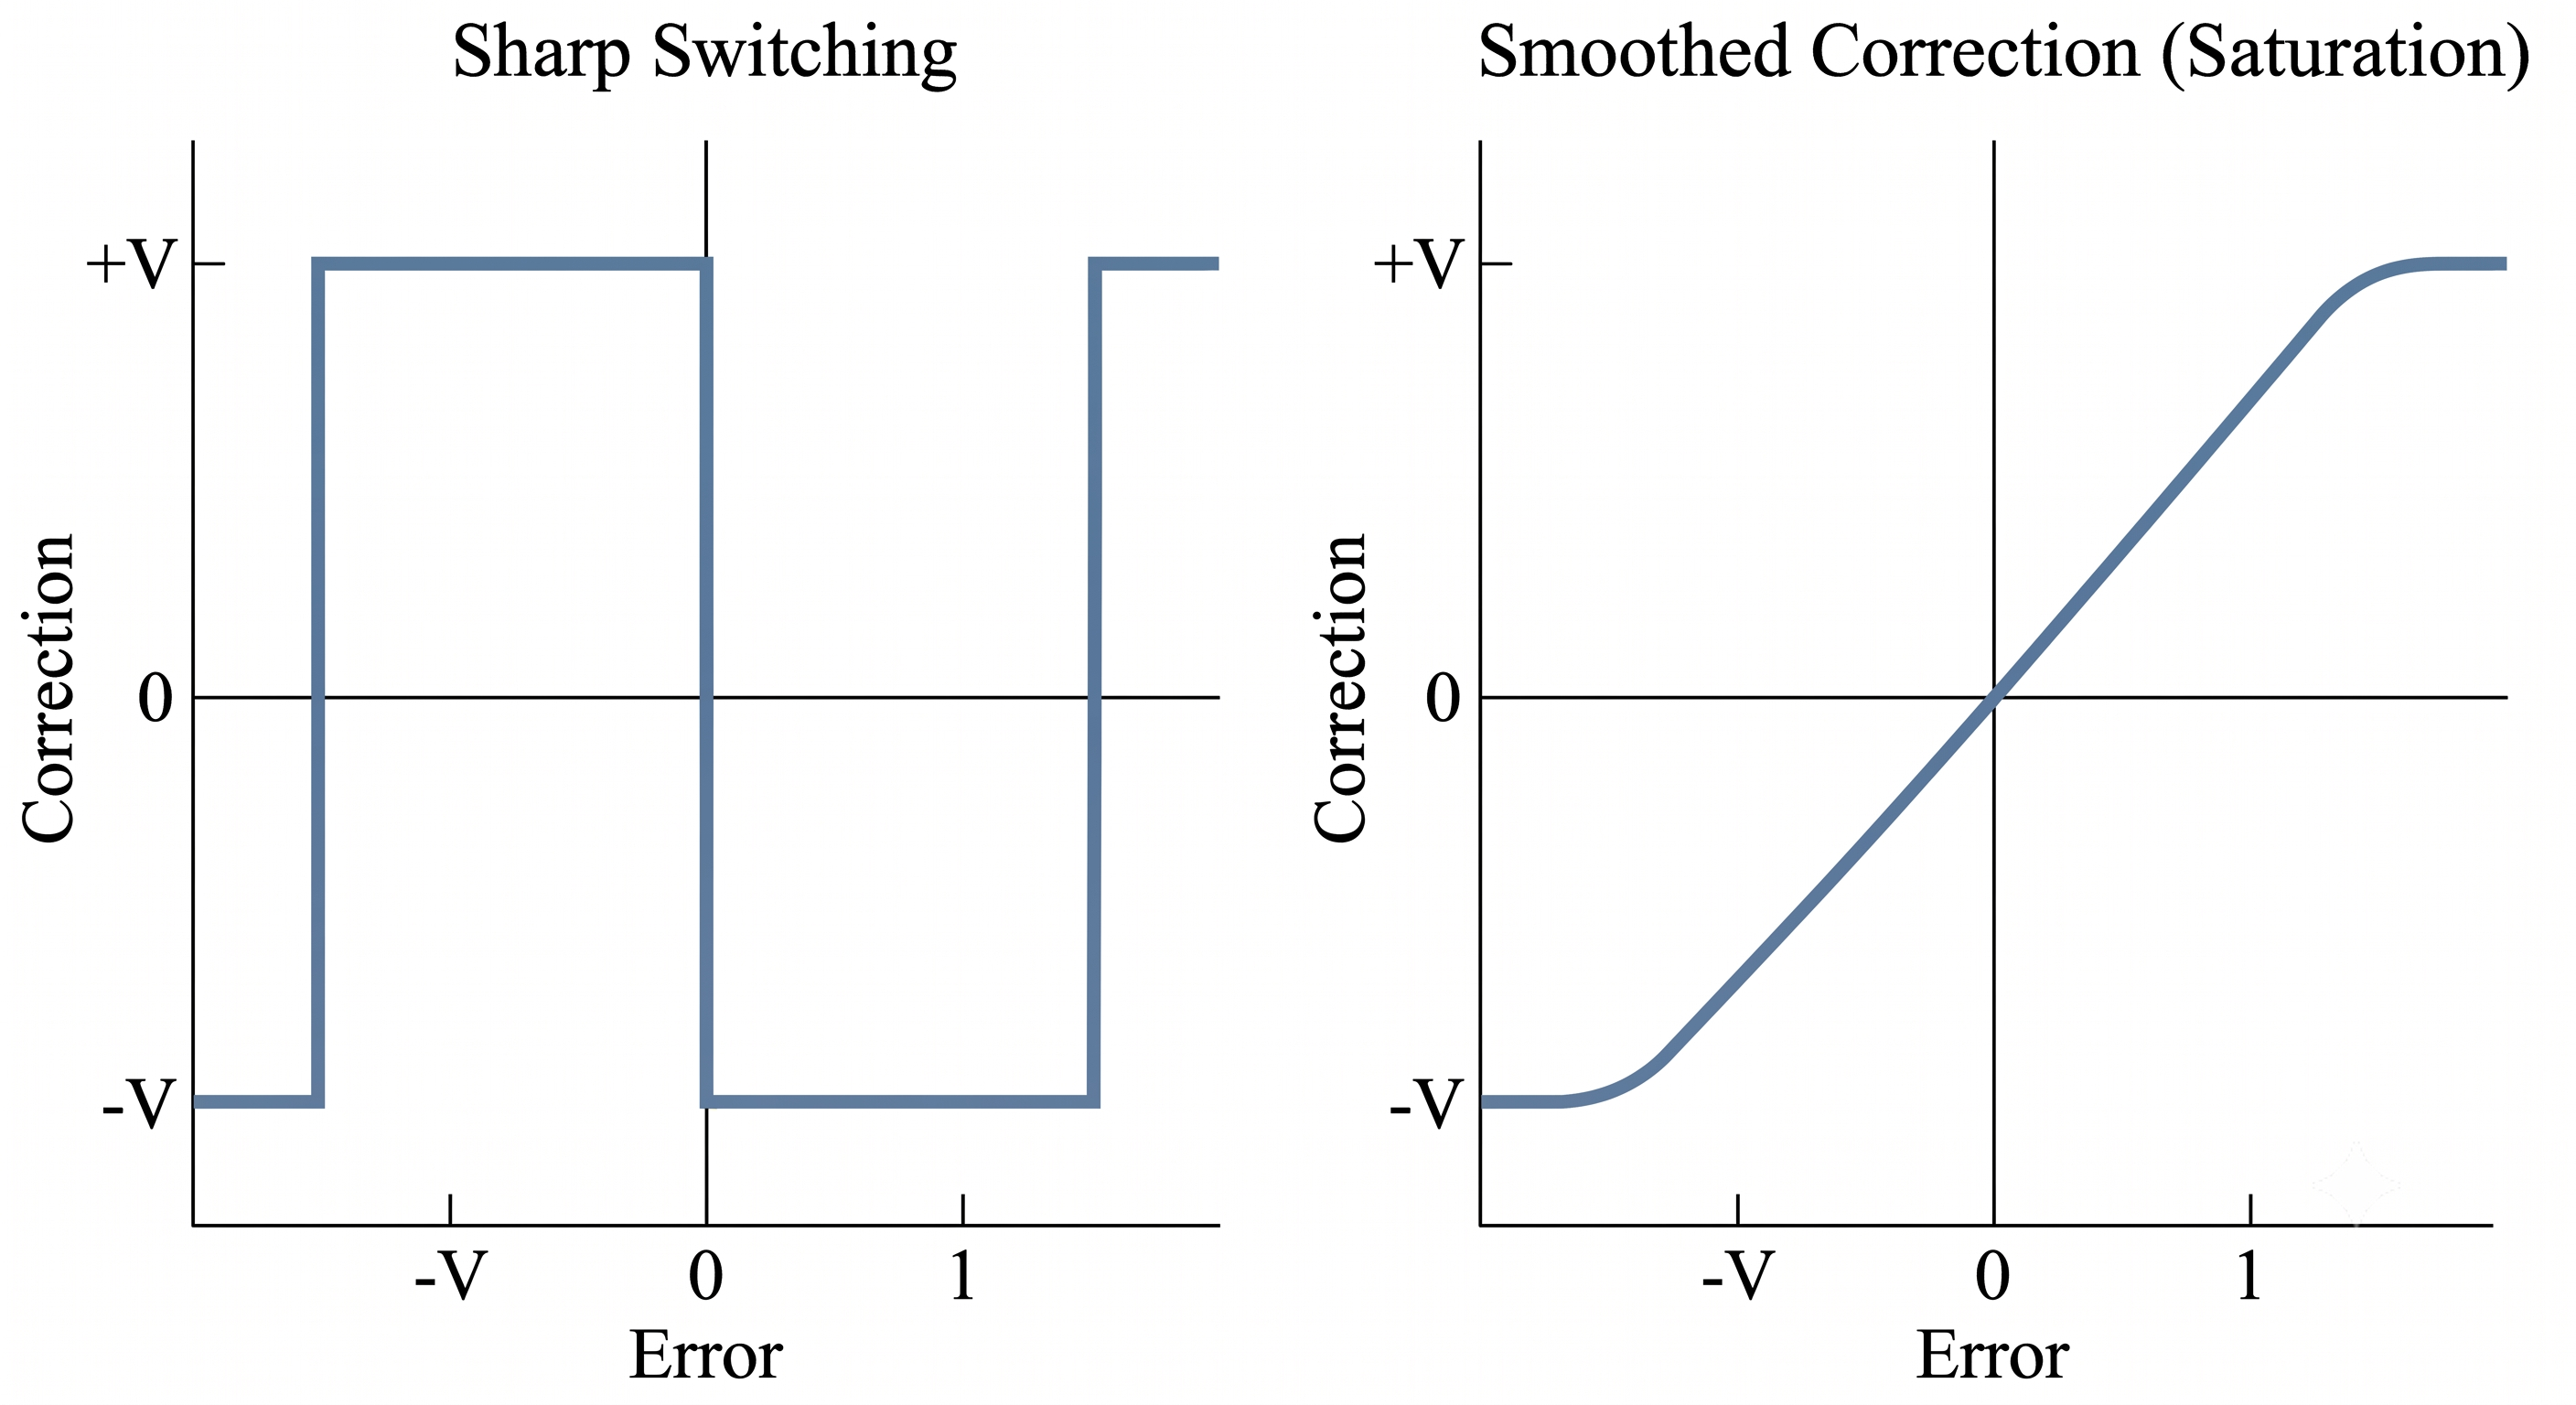
\includegraphics[width=0.85\textwidth]{Gemini_Generated_Image_i8b6zpi8b6zpi8b6.png}
\caption{Sharp switching versus smoothed (saturated) correction: the boundary layer removes the abrupt jump that causes chattering.}
\label{fig:ch6_chattering}
\end{figure}

A small amount of useful information hides inside that switching correction term. Once the estimate has settled, the \emph{average} value of the switching term (obtained simply by smoothing it with a basic low-pass filter) tells us roughly how far off our assumed parameters were -- for example, how much the true ohmic resistance $R_0$ has drifted from its nominal value. This gives sliding mode observers a convenient side benefit: they can be used not just to estimate the hidden voltage, but also to reveal slow, aging-related parameter drift, without needing a separate estimator.

\begin{algorithm}[htbp]

\caption{Sliding Mode Observer with Chattering Suppression}
\label{alg:smo_chattering}

\footnotesize

\begin{algorithmic}[1]

\State \textbf{Input:} Telemetry $\{V_{t,k}, I_k\}$, gains $L, V$, boundary layer width $\epsilon$

\State \textbf{Output:} Estimated polarization voltage $\hat{V}_{1,k}$, smoothed disturbance signal $v_{eq,k}$

\State \textbf{Initialization:} $\hat{V}_{1,0}=0,\ v_{eq,0}=0$

\For{each time step $k$}
    \State Look up the open-circuit voltage: $V_{oc} = \mathrm{lookup\_ocv}(SOC_k)$
    \State Compute the output error: $e_y = (V_{t,k}-V_{oc}) - (-\hat{V}_{1,k}-R_0I_k)$
    \State Compute the smoothed switching correction: $sw = V \cdot \text{sat}(e_y/\epsilon)$
    \State Update the voltage estimate:
    \State $\hat{V}_{1,k+1} = \hat{V}_{1,k} + T_s\left(-\frac{1}{R_1C_1}\hat{V}_{1,k} + \frac{1}{C_1}I_k\right) + L\,e_y + sw$
    \State Smooth the switching signal: $v_{eq,k+1} = v_{eq,k} + \frac{T_s}{\tau_f}(sw - v_{eq,k})$
\EndFor

\end{algorithmic}

\end{algorithm}

Choosing the smoothing time constant $\tau_f$ is another balancing act, similar to the gain trade-off in Table~\ref{tab:ch6_gain_tradeoff}: it must be slow enough to filter out the rapid switching noise, but fast enough to still track real, physical aging trends, which typically develop over minutes to hours rather than seconds. A value of $\tau_f$ between 1 and 5 seconds is a reasonable default for most automotive BMS applications running at a 10~Hz update rate.


\section{Gain-Scheduling and LPV Observers}
\label{sec:lpv_observers}

A single, fixed gain (whether $L$, $K_p$/$K_i$, or $V$) rarely performs equally well across the battery's entire operating range. A gain tuned for a cold, low-charge cell may be too aggressive for a warm, fully-charged one, and vice versa. Instead of designing one single gain, engineers can design a small handful of gains, each tuned for a different operating "corner" (for example: cold and empty, cold and full, hot and empty, hot and full), and then blend between them in real time based on the current state of charge and temperature.

This blending is simply a weighted average. If the measured state of charge and temperature are close to the "hot and full" corner, the observer mostly uses the gain tuned for that corner; if the battery sits between two corners, the observer uses a proportional mix of both. Table~\ref{tab:ch6_lpv_corners} lists the four corners typically used for a lithium-ion cell.

\begin{table}[h!]
\centering
\caption{Typical Operating Corners for a Gain-Scheduled Observer.}
\label{tab:ch6_lpv_corners}
\renewcommand{\arraystretch}{1.3}
\footnotesize
\begin{tabularx}{\textwidth}{|X|c|c|}
\hline
\textbf{Operating Corner} & \textbf{SOC} & \textbf{Temperature} \\
\hline
Cold, low charge & 10\% & 0\textdegree C \\
\hline
Cold, high charge & 90\% & 0\textdegree C \\
\hline
Hot, low charge & 10\% & 50\textdegree C \\
\hline
Hot, high charge & 90\% & 50\textdegree C \\
\hline
\end{tabularx}
\end{table}

The blended, real-time gain is computed with a simple weighted sum:
\begin{equation}
L(t) = \alpha_1(t) L_1 + \alpha_2(t) L_2 + \alpha_3(t) L_3 + \alpha_4(t) L_4
\label{eq:ch6_lpv_blend}
\end{equation}
where $L_1$ through $L_4$ are the four pre-tuned gains for the corners in Table~\ref{tab:ch6_lpv_corners}, and the weights $\alpha_1$ through $\alpha_4$ always add up to 1 and shift smoothly as the battery's actual SOC and temperature move around inside that operating rectangle. When the cell sits exactly at one corner, that corner's gain is used at full weight; when it sits in the middle, all four gains contribute equally.

This approach is attractive for embedded systems because it needs no real-time optimization or heavy matrix math -- only a lightweight weighted average that a low-cost microcontroller can compute in a handful of operations, while still giving the observer a gain that is well-matched to the battery's current operating condition.

% ---------------------------------------------------------------
% Generate this image separately using the prompt below, then save it as:
%   images/ch6_fig4_gain_scheduling_envelope.png
% Prompt:
%   "A simple 2D scatter/rectangle diagram for a textbook: a square
%    plot with horizontal axis 'State of Charge (10%-90%)' and
%    vertical axis 'Temperature (0C-50C)'. The four corners of the
%    square are marked with small labeled dots: 'L1', 'L2', 'L3',
%    'L4'. A single dot somewhere near the middle of the square is
%    labeled 'Current Operating Point' with faint dashed lines
%    connecting it to all four corners, suggesting a weighted blend.
%    Clean, flat vector illustration, pastel color palette, white
%    background, academic textbook figure style."
% ---------------------------------------------------------------
% \begin{figure}[h!]
% \centering
% \includegraphics[width=0.75\textwidth]{images/ch6_fig4_gain_scheduling_envelope.png}
% \caption{Blending observer gains across the operating envelope: the four corner gains are combined based on the current SOC and temperature.}
% \label{fig:ch6_gain_scheduling}
% \end{figure}


\section{Robustness and Convergence: A Practical View}
\label{sec:robustness_convergence}

Formal stability proofs for observers (based on Lyapunov functions and linear matrix inequalities) are important for control-theory research, but for a battery-management engineer the practical takeaway can be summarized without the underlying algebra:

\begin{itemize}
    \item \textbf{Convergence} simply means: if the gains are chosen sensibly (as discussed throughout this chapter), the estimation error will shrink toward zero over time and stay there, rather than growing or oscillating forever.
    \item \textbf{Robustness} means: the observer keeps working reasonably well even when the battery model is not perfectly accurate -- for example, when $R_0$ or $R_1C_1$ have drifted from their nominal values due to aging or temperature.
    \item \textbf{Bounded-error guarantee}: even under the worst realistic disturbances (sensor noise, unmodeled dynamics, fast temperature changes), a well-tuned observer's error stays within a small, predictable range rather than diverging -- it does not need the disturbance to disappear completely, only to stay bounded.
\end{itemize}

In practice, robustness and convergence speed pull in opposite directions, in the same way the gain size did in Table~\ref{tab:ch6_gain_tradeoff}: a more aggressive observer (larger gains, or the switching term of an SMO) converges faster and rejects more disturbance, but is also more sensitive to sensor noise. The right choice depends on the application -- a race-car battery pack that experiences huge, fast current swings may prefer a Sliding Mode Observer's robustness, while a slow-cycling grid-storage battery may be perfectly well served by a simple, low-noise Luenberger observer.

\section{Summary}
\label{sec:ch6_summary}

Observer-based parameter estimation methods provide a deterministic, intuitive alternative to statistical filtering. Table~\ref{tab:ch6_observer_comparison} synthesizes the structural and operational trade-offs across the observer architectures covered in this chapter.

\begin{table}[h!]
\centering
\caption{Comparative Synthesis of Observer Architectures for Battery Parameter Tracking.}
\label{tab:ch6_observer_comparison}
\renewcommand{\arraystretch}{1.3}
\footnotesize
\begin{tabularx}{\textwidth}{|p{2.4cm}|p{1.5cm}|X|p{1.4cm}|}
\hline
\textbf{Observer Architecture} & \textbf{Design Style} & \textbf{Primary Advantage / Limitation} & \textbf{Complexity} \\
\hline
Luenberger Observer & Linear & Low computational cost; sensitive to parameter drift. & Low \\
\hline
PI Observer & Augmented & Compensates steady-state offset; lag in fast dynamics. & Medium \\
\hline
Sliding Mode Observer (SMO) & Switching & Supreme robustness; high-frequency chattering. & High \\
\hline
Gain-Scheduled (LPV) Observer & Adaptive & Matches gain to operating point; needs several pre-tuned gains. & Medium \\
\hline
\end{tabularx}
\end{table}

\subsection{Observer Implementation Guidelines}
Key operational takeaways for BMS software design:
\begin{itemize}
    \item \textbf{Luenberger Observers:} Minimal computational overhead, ideal for baseline state estimation when battery parameters are well calibrated offline and do not drift much.
    \item \textbf{PI Observers:} Effectively eliminate steady-state parameter offsets by remembering and cancelling persistent errors; simple enough to run on ordinary automotive microcontrollers.
    \item \textbf{Sliding Mode Observers:} Deliver the strongest robustness against non-linear dynamics and aging-related model mismatch; the saturation function is essential to avoid chattering in a real embedded system.
    \item \textbf{Gain-Scheduled Observers:} A practical way to get near-optimal performance across the full SOC/temperature range without solving anything online -- just blend a handful of pre-tuned gains.
\end{itemize}

The common thread across all of these observer designs is that they rely on feeding back a simple measurement error rather than tracking complex noise statistics. This makes them attractive for safety-critical battery systems where predictable, easy-to-tune behavior matters as much as raw accuracy. In practice, however, an observer alone cannot fully separate state uncertainty from parameter uncertainty when both are changing at once. The next chapter addresses this more complete co-estimation problem, where states and parameters are tracked together.

This concludes the development of observer-based parameter estimation methods. Next, Chapter~7 explores joint and dual estimation structures where states and parameters are co-estimated simultaneously.